% Created 2024-04-28 Sun 23:53
% Intended LaTeX compiler: pdflatex
\documentclass[presentation]{beamer}
\usepackage[utf8]{inputenc}
\usepackage[T1]{fontenc}
\usepackage{graphicx}
\usepackage{longtable}
\usepackage{wrapfig}
\usepackage{rotating}
\usepackage[normalem]{ulem}
\usepackage{amsmath}
\usepackage{amssymb}
\usepackage{capt-of}
\usepackage{hyperref}
\mode<beamer>{\usetheme{Madrid}}
\definecolor{SUred}{rgb}{0.59375, 0, 0.17969} % SU red (primary)
\definecolor{SUblue}{rgb}{0, 0.17578, 0.38281} % SU blue (secondary)
\setbeamercolor{palette primary}{bg=SUred,fg=white}
\setbeamercolor{palette secondary}{bg=SUblue,fg=white}
\setbeamercolor{palette tertiary}{bg=SUblue,fg=white}
\setbeamercolor{palette quaternary}{bg=SUblue,fg=white}
\setbeamercolor{structure}{fg=SUblue} % itemize, enumerate, etc
\setbeamercolor{section in toc}{fg=SUblue} % TOC sections
% Override palette coloring with secondary
\setbeamercolor{subsection in head/foot}{bg=SUblue,fg=white}
\setbeamercolor{date in head/foot}{bg=SUblue,fg=white}
\institute[SU]{Shenandoah University}
\titlegraphic{\includegraphics[width=0.5\textwidth]{\string~/Documents/suLogo/suLogo.pdf}}
\newcommand{\R}{\mathbb{R}}
\usepackage{tikz}
\usepackage{pgfplots}
\usetheme{default}
\author{Chase Mathison\thanks{cmathiso@su.edu}}
\date{29 April 2024}
\title{General Parabolas}
\hypersetup{
 pdfauthor={Chase Mathison},
 pdftitle={General Parabolas},
 pdfkeywords={},
 pdfsubject={},
 pdfcreator={Emacs 29.1 (Org mode 9.6.7)}, 
 pdflang={English}}
\begin{document}

\maketitle

\section{Announcements}
\label{sec:org8d019ab}
\begin{frame}[label={sec:org16d2903}]{Announcements}
\begin{enumerate}
\item Homework in MyOpenMath due tonight.
\item Exam next week (old exam available in Canvas).
\item Friday's class will be on Thursday this week.
\end{enumerate}
\end{frame}

\section{Lecture}
\label{sec:org46c1550}
\begin{frame}[label={sec:org9629b74}]{General Parabolas}
Let's work out the formula for a general parabola with a vertex at \((h,k)\).

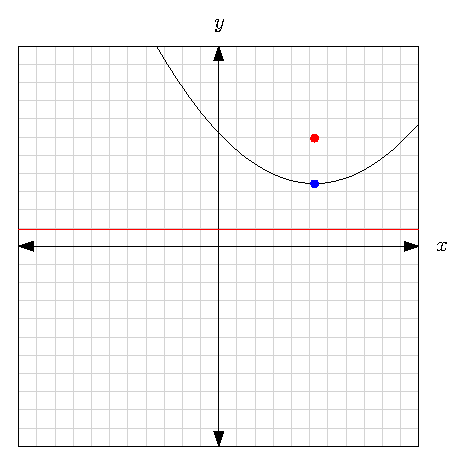
\includegraphics{./general_parabola}
\end{frame}

\begin{frame}[label={sec:org4c71854}]{General Parabolas}
\end{frame}

\begin{frame}[label={sec:org6dd9571}]{Some Information}
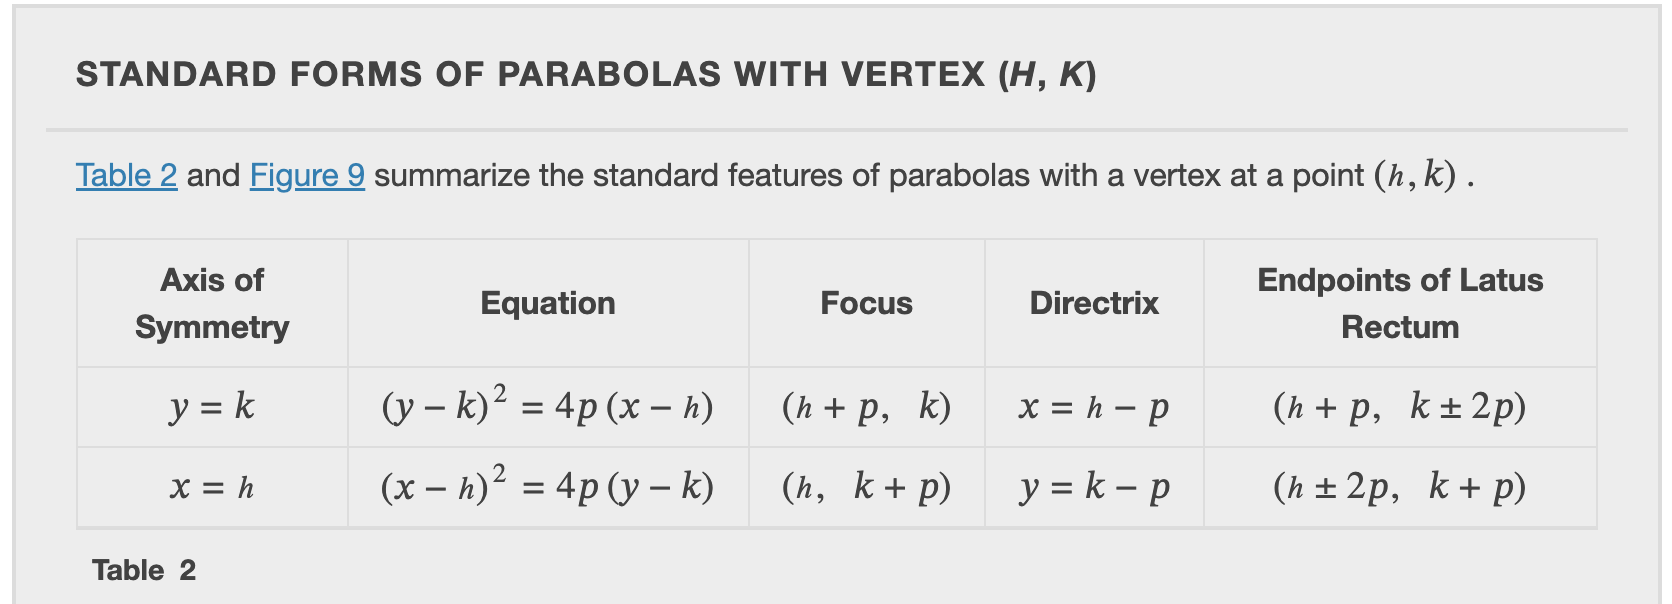
\includegraphics[width=0.9\textwidth]{./parabs_gen}
\end{frame}

\begin{frame}[label={sec:orgbfb227a}]{Example}
Write the equation and graph a parabola that has a focus at \(\left(
1,3 \right)\) and a directrix of \(y = -1.\)

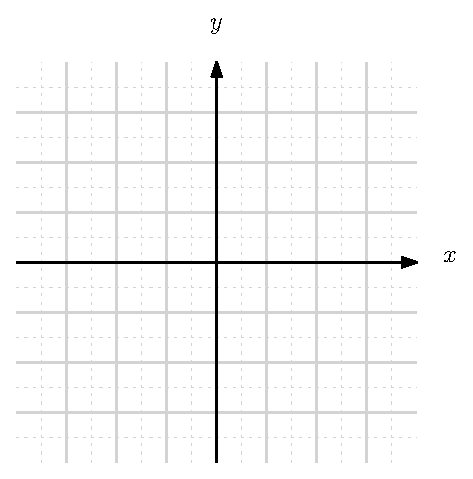
\includegraphics[scale=0.9]{./blank_grid}
\end{frame}

\begin{frame}[label={sec:org6bae603}]{Example}
What are the focus, directrix and vertex for the parabola with equation
\[
y = \frac{x^2}{4}+\frac{5x}{2}+\frac{13}{4}?\]

\vspace{10in}
\end{frame}

\begin{frame}[label={sec:orgc467322}]{Applications of Parabolas}
\end{frame}

\begin{frame}[label={sec:orgd34c962}]{Example}
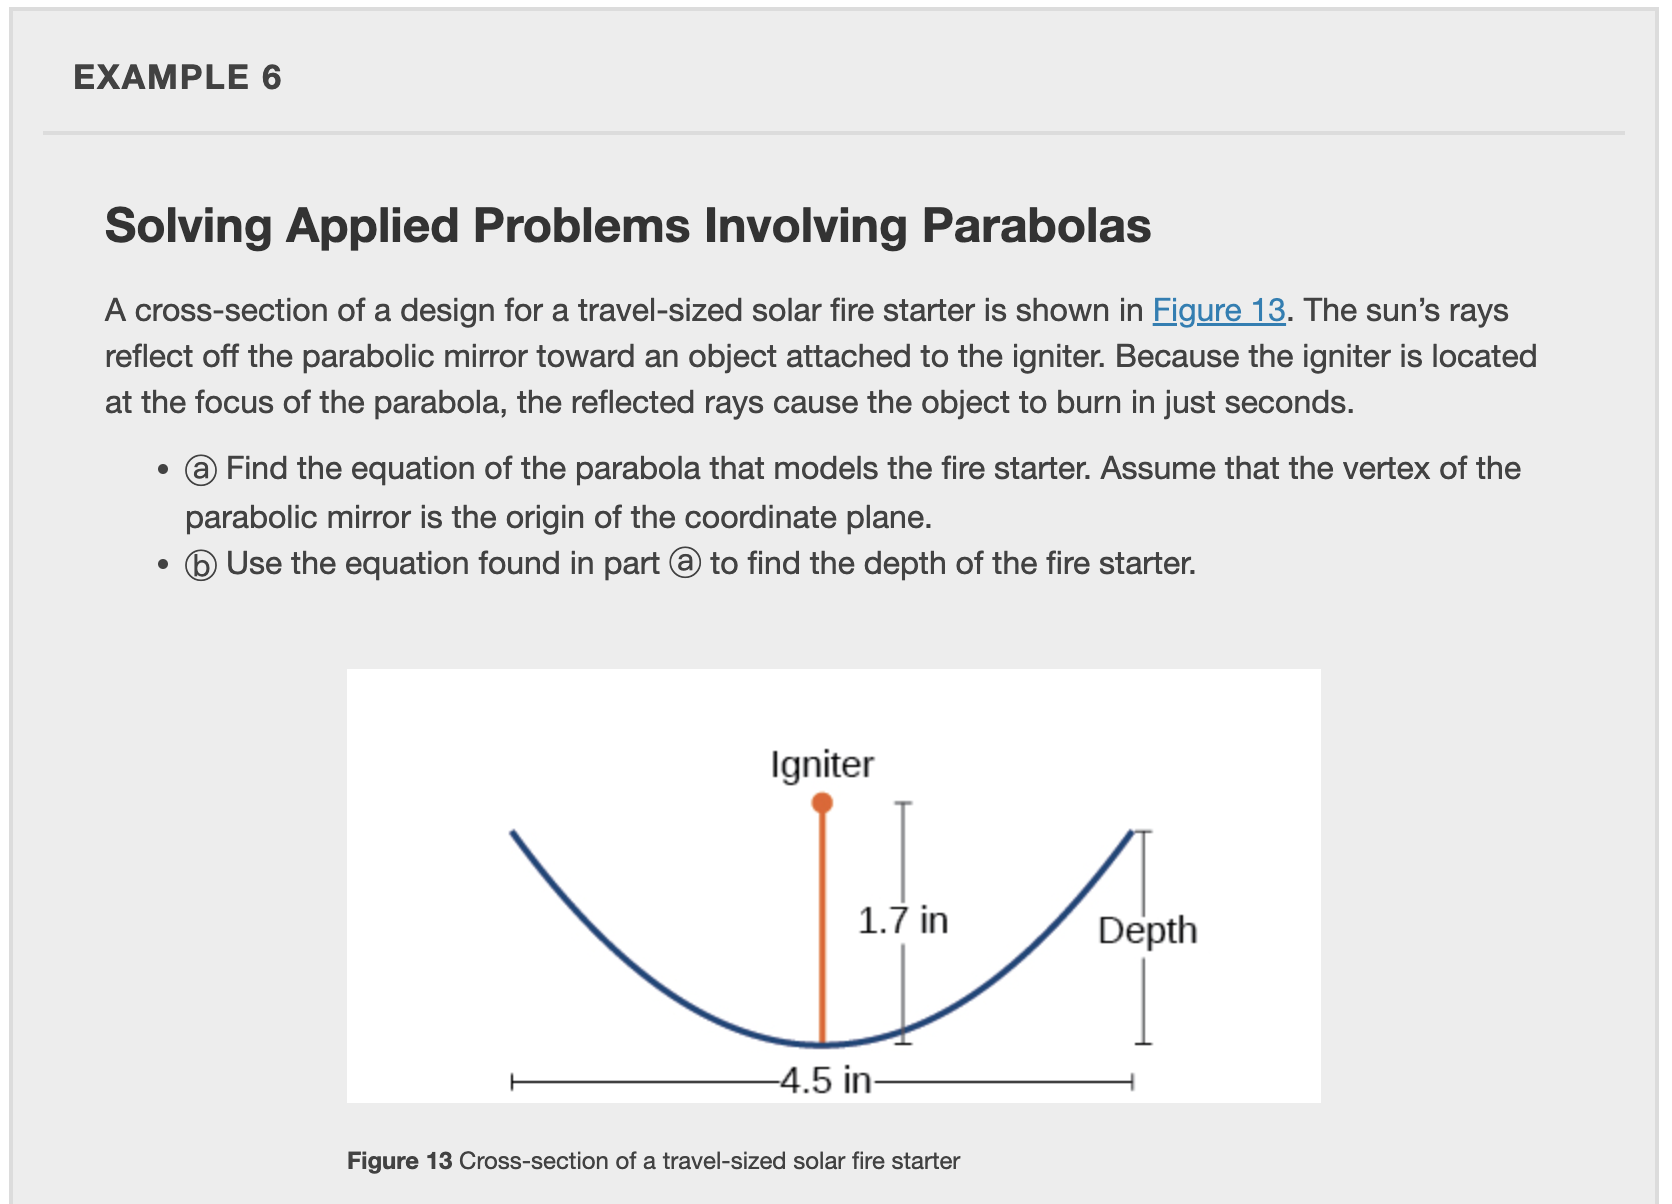
\includegraphics[width=0.8\textwidth]{./applied_parab}
\end{frame}

\begin{frame}[label={sec:orga15a791}]{Example}
\end{frame}
\end{document}